
\documentclass[10pt,letterpaper]{article}



% Some useful packages
% math
\usepackage{amsmath}
% pretty colors
\usepackage{color}
% nicer urls that break at the end of the page
\usepackage{url}
% every document needs images
\usepackage{graphicx}
\usepackage{setspace}

\graphicspath{{./figures/}}   % where to look for images

%let's fiddle with the default margins to save some trees
%this makes the odd side margin go to the default of 1inch
\oddsidemargin 0.0in
%sets the textwidth to 6.5, which leaves 1 for the remaining right margin with 8 1/2X11inch paper
\textwidth 6.5in
% less white space, please!
\headheight 0.0in
% shift everything up
\topmargin -0.5in
\footskip .6in
% text should take up all but a 1'' margin
\textheight 9.0in
\doublespacing


% Define some shortcuts for things I want to use.
% Use them like, for example:
% \begin{hypothesis}Lettuce causes brain damage.\end{hypothesis}
% Numbering & formatting will happen automatically.
\newtheorem{hypothesis}{Hypothesis}
\newtheorem{task}{Task}
\newtheorem{contribution}{Contribution}


% Shortcuts: allows you to use limited markup when editing/collaborating.
% \comment{This section needs to be rewritten.}
\def\ask#1{\textcolor{red}{\bf $\langle\langle$Question:\ #1$\rangle\rangle$}}
\def\comment#1{\textcolor{red}{\bf $\langle\langle$Comment:\ #1$\rangle\rangle$}}


% This imitates the Wikipedia ``Citation Needed'' text; use it as a temporary
% marker for things you need to cite.
\def\citationneeded{$^{\textcolor{blue}{\text{[citation needed]}}}$ }

% format et al.
\def\etal{\textit{et al.}}
\def\ie{\textit{i.e.}}
\def\eg{\textit{e.g.}}

\title{Attempts to exercise in Reinforcement Learning book Chapter 2}
\author{Mengliao Wang}


\begin{document}

% Generate Title Page
\maketitle

% these makes the title page be only a title page, the paper will start on the next page.
% Remove it to save even more trees.
\thispagestyle{empty}
\clearpage

% this dumps the abstract on a front page all by itself.

\section*{Exercise 2.1: }
\label{2.1}

Given enough steps per run, the greedy approach will remain as the reward of 1. However both approaches with $\varepsilon=0.1$ and $\varepsilon=0.01$ will reach the optimal $Q_t(a)$ so that $Q_t(a)=q_*(a)$ by the law of large numbers. However since the $\varepsilon=0.1$ method will always make 10\% of exploration moves, the cumulative probability will be around 90\%. While the cumulative probability for the $\varepsilon=0.01$ approach will be around 99\%. Regarding rewards it will be more complicated to calculate, as the $q_*(a),a=1,..,10$ is randomly decided based on a normal distribution. Suppose the action with highest $q_*(a)$ is $a=1$ (the order of the actions can be switched in arbitrary way), with $q_*(a=1)=m$ and $\sum\limits_{k=2}^{10}q_*(a=k) = n$. The $\varepsilon=0.1$ approach will eventually have the reward of $0.9m+0.1n/9$, while the $\varepsilon=0.01$ approach will eventually have the reward of $0.99m+0.01n/9$.

\section*{Exercise 2.2: }
\label{2.2}
\begin{align}
Q_{n+1}&=Q_n+\alpha_n(R_n-Q_n)\\
&= \alpha_nR_n + (1-\alpha_n)(Q_{n-1}+\alpha_{n-1}(R_{n-1}-Q_{n-1})\\
&= \alpha_nR_n + (1-\alpha_n)\alpha_{n-1}R_{n-1}+(1-\alpha_n)(1-\alpha_{n-1})Q_{n-1}\\
&= \alpha_nR_n + (1-\alpha_n)\alpha_{n-1}R_{n-1} + (1-\alpha_n)(1-\alpha_{n-1})\alpha_{n-2}R_{n-2} + ... + (\prod_{i=1}^{n-1}(1-\alpha_{n-i+1}))\alpha_1R_1+(\prod_{i=1}^{n}(1-\alpha_{n-i+1}))Q_1
\end{align}

So the weight for each reward k would be $(\prod_{i=1}^{n-k}(1-\alpha_{n-i+1}))\alpha_k$. When we replace $\alpha_n$ to be a constant, we would have the same result as formula (2.6).

\section*{Exercise 2.3: \textit{Programming} }
\label{2.3}
*Source code to be attached.
\begin{figure}[htp]
  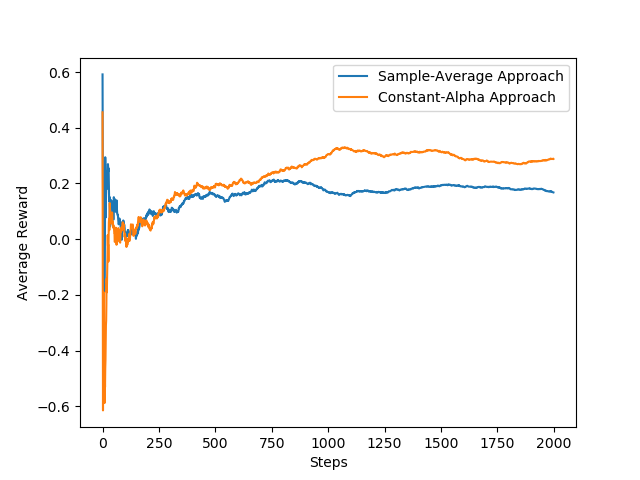
\includegraphics[width=0.5\textwidth]{Reward-var-001}
  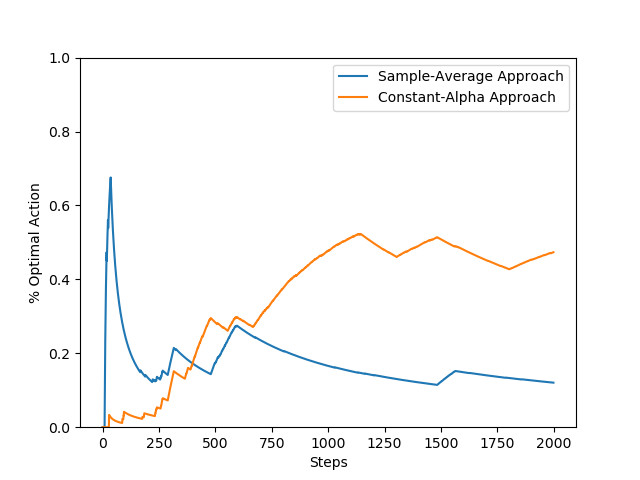
\includegraphics[width=0.5\textwidth]{Perc-var-001}
  \caption{Reward and \% Optimal Action for random walk variance = 0.01}
  \label{fig:var-001}
\end{figure}

\begin{figure}[htp]
  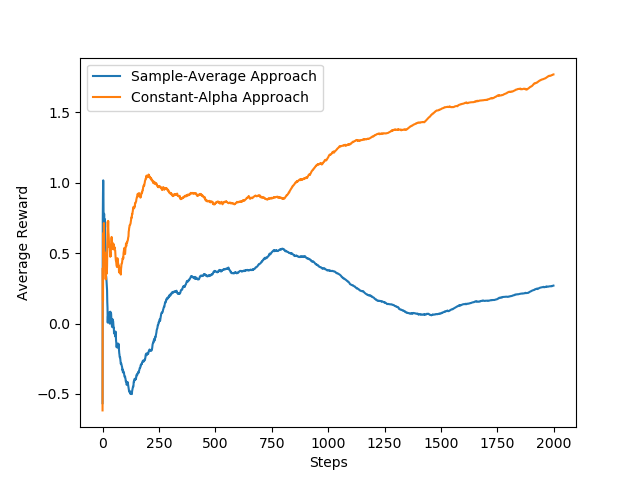
\includegraphics[width=0.5\textwidth]{Reward-var-01}
  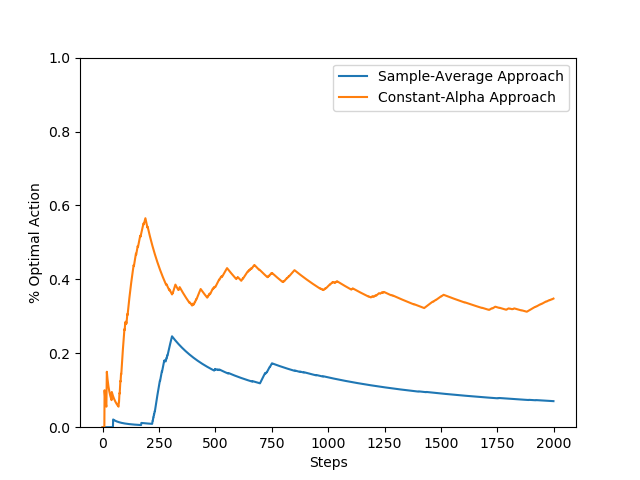
\includegraphics[width=0.5\textwidth]{Perc-var-01}
  \caption{Reward and \% Optimal Action for random walk variance = 0.1}
  \label{fig:var-01}
\end{figure}
The results have been shown in Figure \ref{fig:var-001} and Figure \ref{fig:var-01}. In Figure \ref{fig:var-001} the mean value for each bandit arm is updated based on a random number drawn from normal distribution $\mathcal{N}(0,\,0.01)$. Here the Constant-Alpha approach is better than the Sample-Average approach, because the Constant-Alpha approach will keep a bigger weight on the recent rewards. Also as expected, when we increase the distribution variance of the random walk variable to 0.1 as shown in Figure \ref{fig:var-01}, the Constant-Alpha approach is more significantly better than the Sample-Average approach. It might be because the hidden $q_*(a)$ are oscillating stronger than the previous experiment by each time step, which makes the history less useful and thus reduces the performance of sample-average approach further more. The Constant-Alpha remains on a relatively good level, even when the task is obviously more difficult than the previous task with variance as 0.01.



\section*{Exercise 2.4:}
\label{2.4}

There were oscillations and spikes at the beginning because the value function is very sensitive to any change in the rewards at the early stage. Since $Q_1=5$ is out of the confidence interval of $q_*(a)$, after 10 runs all the value function will be reset to close to each $q_*(a)$, which are supposed to be having means around 0. When there is a significant different between the best bandit k and the other nines, $Q_k$ would be quickly stacking up and make the percentage of optimal calls much higher. To the opposite, if there is not such a difference between the real distributions $q_*(a)$, the learning process will be based on the random sampling, which are relatively much smaller values, so it is harder to make a optimal call.

\section*{Exercise 2.5: }
\label{2.5}

At the first 10 steps, each action will be randomly visited one by one since $N_t(a)=0, a=1,2,..,10$. Thus the reward will be an average of 10 action sampling results, which is close to be around 0. By step 11, the action selection will be based on $Q_t(a)+c\sqrt{\dfrac{\log t}{N_t(a)}}$. Given $c=2, t=11, N_t(a)=1$, the second part of the equation is about 2.04. For step 11 the second part is the same for all actions, so we will select the action with the highest reward $R_t(a)$. Thus only at step 11 the algorithm is doing a full exploitation instead of full exploration, and that's why there is a spike here. After step 11 all the other 9 actions that were not picked will have value of roughly 2.08 for the second part of the expression $c\sqrt{\dfrac{\log t}{N_t(a)}}$, while the one that got picked will have a value of 1.76. Also the first part $Q_t(a)$ will be picked from the distribution with mean value in a $\mathcal{N}(0,\,1)$, so the exploration is again making a dominant effect (not a full exploration as in the first 10 steps though). That's why we saw the reward decreases after step 11.
\clearpage

\end{document}
